%%%%%%%%%%%%%%%%%%%%%%%%%%%%%%%%%%%%%%%%%%%%%%%%%%%%%%%%%%%%%%%%%%%%%%%%%%%%%%%
% name:         | http.tex
% @uthor:       | Maxime Fourcade <maxime.fourcade@eisti.fr>
% title:        | Include : HTTP
% brief:        | Explications du protocole HTTP pour la Coding Night du 12/11
% licence:      | free
% more:         | Warning: inputenc en utf8
%               | Warning: n'oublies pas vos \subsection (3 à 4 maximum)
%%%%%%%%%%%%%%%%%%%%%%%%%%%%%%%%%%%%%%%%%%%%%%%%%%%%%%%%%%%%%%%%%%%%%%%%%%%%%%%


\section{Le protocole HTTP}
\begin{frame}\frametitle{}
    {\Huge Le protocole HTTP}

    \vspace{2em}

    Le net c'est bien, mais comment ça marche ?
\end{frame}



\subsection{Introduction}

\begin{frame}{Qu'est ce qu'un protocole ?}


\textbf{\huge Comment font deux machines pour communiquer ?} \\

\vspace{1em}
		
\begin{itemize}

	\item Règles et spécifications : normes
	\item Etapes de communication
	\item Couches de protocoles : Modèle OSI

\end{itemize}




\end{frame}{}

\begin{frame}{Modèle \textbf{O}pen \textbf{S}ystem \textbf{I}nterconnection : \textbf{OSI}}

    \begin{center}
        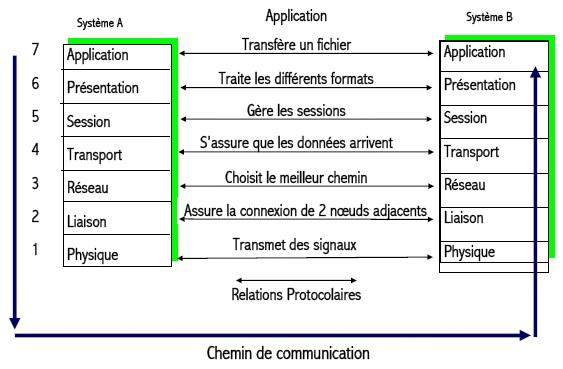
\includegraphics[width=0.9\textwidth]{img_http/OSI.jpg}
    \end{center}

\end{frame}




\subsection{Description}

\begin{frame}{Protocole HTTP}
	
	\begin{center}

		{\Large \textbf{H}yper\textbf{T}ext \textbf{T}ransfert \textbf{P}rotocol}  \vspace{2em}

		\begin{itemize}
			\item Communication : Client $\leftrightarrow$ Serveur\\
			\item Protocole de couche Application, fonctionne sur n'importe quelle connexion\\
			\item Version sécurisée : HTTPS par SSL / TLS
			\item Votre navigateur web est un client HTTP
			\item Serveurs HTTP : Apache, IIS (Microsoft), NodeJS, GWS (Google)
		\end{itemize}
	\end{center}

\end{frame}



\subsection{Historique}


\begin{frame}{C'est vieux HTTP ?}
	
Son inventeur : \emph{Tim Berners-Lee} en 1990 - président de W3C. \vspace{1em}

3 principales technologies du Web :
\begin{itemize}
\item HTTP : tel que nous le voyons en ce moment
\item URL : adresses Web
\item HTML : HyperText Markup Language
\end{itemize}
\vspace{1em}

V0.9 : Seuls les fichiers HTML sont supportés.

V1.0 : Type MIME supporté.

V1.1 : Performances et supports améliorés.

\end{frame}



\subsection{Implémentation}


\begin{frame}{Comment ça marche ?}

\begin{center}
\textbf{\large Système de requêtes / réponses}.

\vspace{1em}

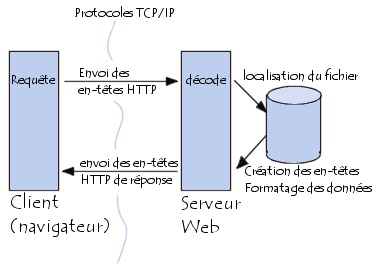
\includegraphics[scale=0.75]{img_http/schema_http.jpg}
\end{center}

\end{frame}


\subsubsection{Requêtes}


\begin{frame}{Comment faire une requête ?}
	
    \begin{center}
        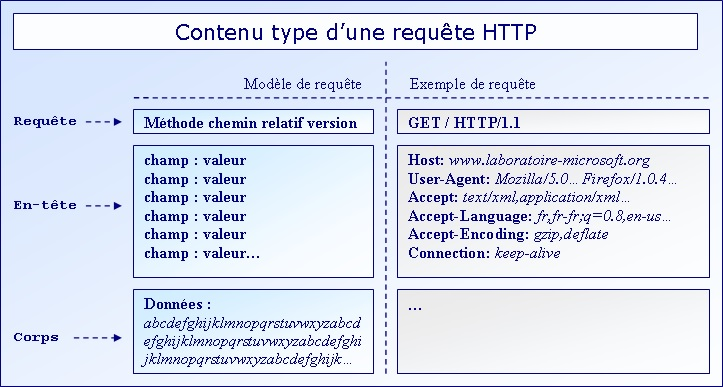
\includegraphics[width=1\textwidth]{img_http/requete.jpg}
    \end{center}

\end{frame}


\begin{frame}{Méthodes}

Liste des méthodes les plus connues :

\vspace{2em}

\begin{table}[h]
\begin{tabular}{|l|l|}
\hline
   Commande & Description\\ \hline \hline
   \textbf{GET} & Requête de la ressource située à l'URL spécifiée\\ \hline
   \textbf{HEAD} & Requête de l'en-tête de la ressource située à l'URL\\ \hline
   \textbf{POST} & Envoi de données au programme situé à l'URL\\ \hline
   \textbf{TRACE} & Retourne les données envoyés sans traitement à l'URL\\ \hline
   \textbf{PUT} & Envoi de données à l'URL\\ \hline
   \textbf{PATCH} & Modification partielle de la ressource située à l'URL\\ \hline
   \textbf{DELETE} & Suppression de la ressource située à l'URL\\ \hline
\end{tabular}
\end{table}

\end{frame}


\begin{frame}{En-têtes}

\begin{table}[h]
    \begin{tabular}{|l|p{0.65\textwidth}|}
\hline
   En-tête & Description\\ \hline \hline
   \textbf{Host} & Nom de domaine du site Web\\ \hline
   \textbf{User-Agent} & Application envoyant la requête\\ \hline
   \textbf{Accept} & Type de contenu accepté par le client\\ \hline
   \textbf{Accept-Charset} & Jeux de caractères supportés par le client\\ \hline
   \textbf{Content-Encoding} & Type de codage de la requête\\ \hline
   \textbf{Content-Length} & Taille du corps de la requête\\ \hline
   \textbf{Content-Type} & Type de contenu du corps de la requête\\ \hline
   \textbf{Connection} & Indique si les connexions sont persistantes\\ \hline
   \textbf{Date} & Date de début de transfert des données\\ \hline   
   \textbf{Refer} & Page actuelle affichée sur le client\\ \hline
   \textbf{Cookie} & Nom et valeurs des cookies associés\\ \hline
\end{tabular}
\end{table}

\end{frame}

\subsubsection{Réponses}

\begin{frame}{Et maintenant une réponse ?}
	
    \begin{center}
        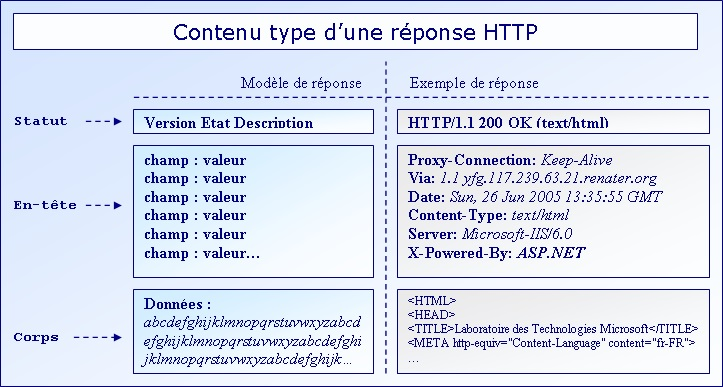
\includegraphics[width=1\textwidth]{img_http/reponse.jpg}
    \end{center}

\end{frame}



\begin{frame}{Codes de réponse}

La réponse renvoie obligatoirement un code :
\begin{itemize}
   \item \textbf{1xx} : Messages d'information
   \item \textbf{2xx} : Succès de la requête
	\begin{itemize}
		\item 200 : OK
		\item 201 : Created
		\item 202 : Accepted
	\end{itemize}
   \item \textbf{3xx} : Redirection de la ressource
   \item \textbf{4xx} : Erreur due au client
	\begin{itemize}
		\item 400 : Bad Request
		\item 403 : Forbidden
		\item 404 : Not Found
	\end{itemize}
   \item \textbf{5xx} : Erreur due au serveur
	\begin{itemize}
		\item 503 : Service Unavailable
		\item 505 : HTTP Version Not Supported
	\end{itemize}
\end{itemize}

\end{frame}


\begin{frame}{En-têtes}

\begin{table}[h]
\begin{tabular}{|l|l|}
\hline
   En-tête & Description\\ \hline \hline
   \textbf{Content-Encoding} & Type de codage du corps de la réponse\\ \hline
   \textbf{Content-Language} & Type de langage du corps de la réponse\\ \hline
   \textbf{Content-Length} & Longueur du corps de la réponse\\ \hline
   \textbf{Content-Type} & Type de contenu du corps de la réponse\\ \hline
   \textbf{Date} & Date de début de transfert des données\\ \hline   
   \textbf{Expires} & Date limite de consommation des données\\ \hline
   \textbf{Server} & Caractéristiques du serveur émetteur\\ \hline
\end{tabular}
\end{table}

\end{frame}

